\chapter{Second Order Linear Ordinary Differential Equations \ode{}s}

\begin{example}[Checking for Linearity] Determine which of the following systems are linear:
\begin{fullwidth}
\begin{colenumerate}[3]
\item
\begin{align}
\dot x_1 = x_2ta \\
\dot x_2 = x_1+b
\end{align}
\item
\begin{align}
\dot x_1 = t^2x_2a\\
\dot x_2 = x_1 + bx_2
\end{align}
\item
\begin{align}
\dot x_1 = ax_1x_2\\
\dot x_2 = x_1+bx_2
\end{align}
\end{colenumerate}
\end{fullwidth}
\end{example}

\textbf{Solution} 

Recall from last class that an ODE
\begin{equation}\label{eq: gen ode}
\underline {\dot x} =f(\underline x, t;\underline a)
\end{equation}
is a linear function of state $x$ if it satisfies the following:

\begin{compactitem}
\item Additivity:  $f(\underline x_1+\underline x_2, t;\underline a) = f(\underline x_1, t; \underline a)+f(\underline x_2,t;\underline a)$
\item Homogeneity: $f(c\cdot \underline x, t;\underline a) = c\cdot f(\underline x, t; \underline a)$,  $\forall c \in \mathbb R $.
\end{compactitem}

Now consider the three systems of ODE's - notice that: 
\begin{compactenum}
\item  the first system, equation (2) does not pass through the origin (0,0), thus we can readily conclude that the system is nonlinear.
\item  the second system satisfies both additivity and homogeneity and is in fact a linear system. 
\item the third system is not a linear system due to the $x_1x_2$ term in equation (5). 
\end{compactenum}

\newthought{Direct Consequences of Linearity}
\begin{compactenum}
\item  linear systems have the origin as an equilibrium point.
 $$f(0, t;\underline a) = f(\underline x - \underline x, t; \underline a) = f(\underline x, t; \underline a)-f(\underline x,t;\underline a)$$
\item $x_1^*, x_2^*$ are equilibria such that 
$$F(\alpha x_1^* + \beta x_2^*, t;\underline a) = \alpha F( x_1^*, t; \underline a) + \beta F(x_2^*, t; \underline a)$$
This means that a linear system will have at minimum a single equilibrium point, the origin. Should the system have two equilibrium points, we are able to create infinitely many equilibrium points using linear combinations of the the two (or more) points. 
\begin{figure}
  \centering
  \includegraphics[width=0.4\linewidth]{figs/line-eqpts.png}  
  \caption{Illustration of how we can use two equilibrium points, $a$ and $b$ to create a line of infinitely many equilibrium points.}
\end{figure}

When we consider that a system of ODE's can have infinitely many equilibrium points by way of linear recombinations, it doesn't make sense to ask \textit{how many} equilibrium points a system has, instead, it is of interest to ask  \textit{What is the dimension of the subspace the equilibrium points are on?} Do the equilibrium points span a line, a plane, or surface? 
\end{compactenum}

\newthought{Eigenvalues and Eigenvectors}
Suppose we have a differential equation of the form 
$$ \dot x = A \underline x$$ 
Assume $(\lambda, \nu)$ such that $A \nu = \lambda \nu$. Each eigenvector corresponds to a simple solution of the form $x(t) = c(t) \nu$. We use substitution to write the following:

\begin{align}
\dot x &= A c(t) \nu \\
\dot c(t) \nu &=  A c(t)  \nu \\
\dot c(t) \nu &=  c(t) \lambda \nu \\
\dot c(t) &=  c(t) \lambda \\
c(t) &=  c(0) e^{\lambda t}
\end{align}

In general, solutions will take the form  $x_k(t) = ce^{\lambda t} \nu_k$. If $x \in \mathbb{R}^N$ and the matrix A has $N$ eigenvectors, then we say the set of eigenvectors is \textbf{complete} and solutions take the form
\begin{align}
     \underline{x}(t) = \sum_{k=1}^{N} c_k e^{\lambda_k t}\nu_k
\end{align}
where $\nu \in \mathbb(C)^k$

To write the solutions of $\underline{x}(t)$, note that if we have a complete, or linearly independent, set of eigenvectors, we can write them in an orthogonal and non-singular matrix $P$. 
\begin{align}
    P = [\nu_1,\nu_2,\nu_3,...,\nu_n]
\end{align}
Then we can express the solutions for $\dot x$ as  
\begin{align}
     \underline{x}(t) = P \Lambda(t) \underline{c} 
\end{align}
 such that
\[
\underbrace{
\begin{bmatrix}
  x_1(t) \\  x_2(t)  \\ . \\ .  \\ .  \\ x_{n-1}(t) \\ x_{n}(t)
\end{bmatrix}}_{\underline{x}(t)} =
\underbrace{
\begin{bmatrix}
  . &. &. &. & .&. &. &.  \\. &. &. &. & .&. &. &.  \\  . &. &. &. & .&. &. &. \\ v_{1} &v_{2} &. &. & .&. &v_{n-1} &v_{n} \\ . &. &. &. & .&. &. &. \\ . &. &. &. & .&. &. &. \\ . &. &. &. & .&. &. &.
\end{bmatrix}
}_{P}\cdot 
\underbrace{
\begin{bmatrix}
  e^{\lambda_{1}t} &. &. &. & .&. &. &.  \\  . & e^{\lambda_{2}t} &. &. & .&. &. &. \\  . &. &. & .&. &.&. \\ . &. &. &. & .&. &. &.  \\ . &. &. &. & .&. &. &. \\ . &. &. &. & .&. &e^{\lambda_{n-1}t} &. \\ . &. &. &. & .&. &. &e^{\lambda_{n}t} 
\end{bmatrix}}_{\Lambda} \underbrace{
\begin{bmatrix}
  c_1 \\  c_2  \\ . \\ .  \\ .  \\ c_{n-1}  \\c_{n} 
\end{bmatrix}}_{\underline{c}}
\] We can determine the value of $\underline{c}$ by computing $$ \underline{x}(0) = P \Lambda(0) \underline{c} = PI \underline{c}$$ where $I$ is the identity matrix. Then  \begin{align}
    \underline{c} = P^{-1}\underline{x}(0)
\end{align} 

and the solution to the system of ordinary differential equations can be written: 

\begin{align}
    \underline{x}(t) = P \Lambda (t) P^{-1}\underline{x}(0)
\end{align}

We define the \textbf{exponential matrix} as $$ \Phi (t)= P \Lambda (t) P^{-1} $$ If a matrix has a complete set of eigenvectors we define 

\begin{align}
    e^{at} = \sum_{n=0}^{\infty} \frac{ A^n t^n}{n!} = P \Lambda (t) P^{-1} 
\end{align} 

\begin{example}[The Simplest Case] Consider the first order differential equation $ \dot s = \lambda s$. From differential equations, we know that the solution to the ODE is has the form $ s(t) =s(0)e^{\lambda t}$
\end{example}

What we've accomplished in class is show that the form we are familiar with in the simplest of differential equations, extends to more complex systems of differential equations. 
\begin{align}
\dot x &= A \underline{x} \\
\underline{x}(t) &= \Phi (t) \underline{x}(0) = e^{at}\underline{x}(0)
\end{align} 


%%% Local Variables:
%%% mode: latex
%%% TeX-master: "main"
%%% End:














\section{Characteristic Equation, Complex numbers}

\begin{weekintro}
  Higher-order \ode{}s\index{\ode{}!higher order} often serve as models for mechanical and electrical systems, as relationships between position/velocity/acceleration and charge/current/voltage require multiple derivatives.

  Characteristic\index{characteristic equation!higher order \ode{}s} equations\footnote{``Characteristic'' and ``auxiliary'' equations are used interchangeably here and in the textbook. We will see that another characteristic equations will appear in matrix \ode{}s, and its roots are going to carry a similar interpretation.} help us solve higher-order linear \ode{}s whose parameters (coefficients) do not change. They convert a \ode{} into a polynomial equation, whose roots help us write down the solution. As polynomials can have complex numbers as roots, we will have to learn basic complex number arithmetic.

  Complex numbers\index{complex numbers} \(z \in \mathbb{C}\) are specified using two (independent) real numbers (elements of \(\mathbb{R}\)). There are two different representations of any complex number \(z\):
  \begin{description}
  \item[Cartesian] \(z = \Re z + i \Im z\) \\
    Components are called real and imaginary parts. \index{complex number!cartesian form}
  \item[Polar] \(z = \abs{z} e^{i \arg(z)}\) \\
    Components are called magnitude (or modulus) and angle (or argument). \index{complex number!polar form}
  \end{description}
\end{weekintro}

\subsection*{Homework}
\begin{marginfigure}\centering
  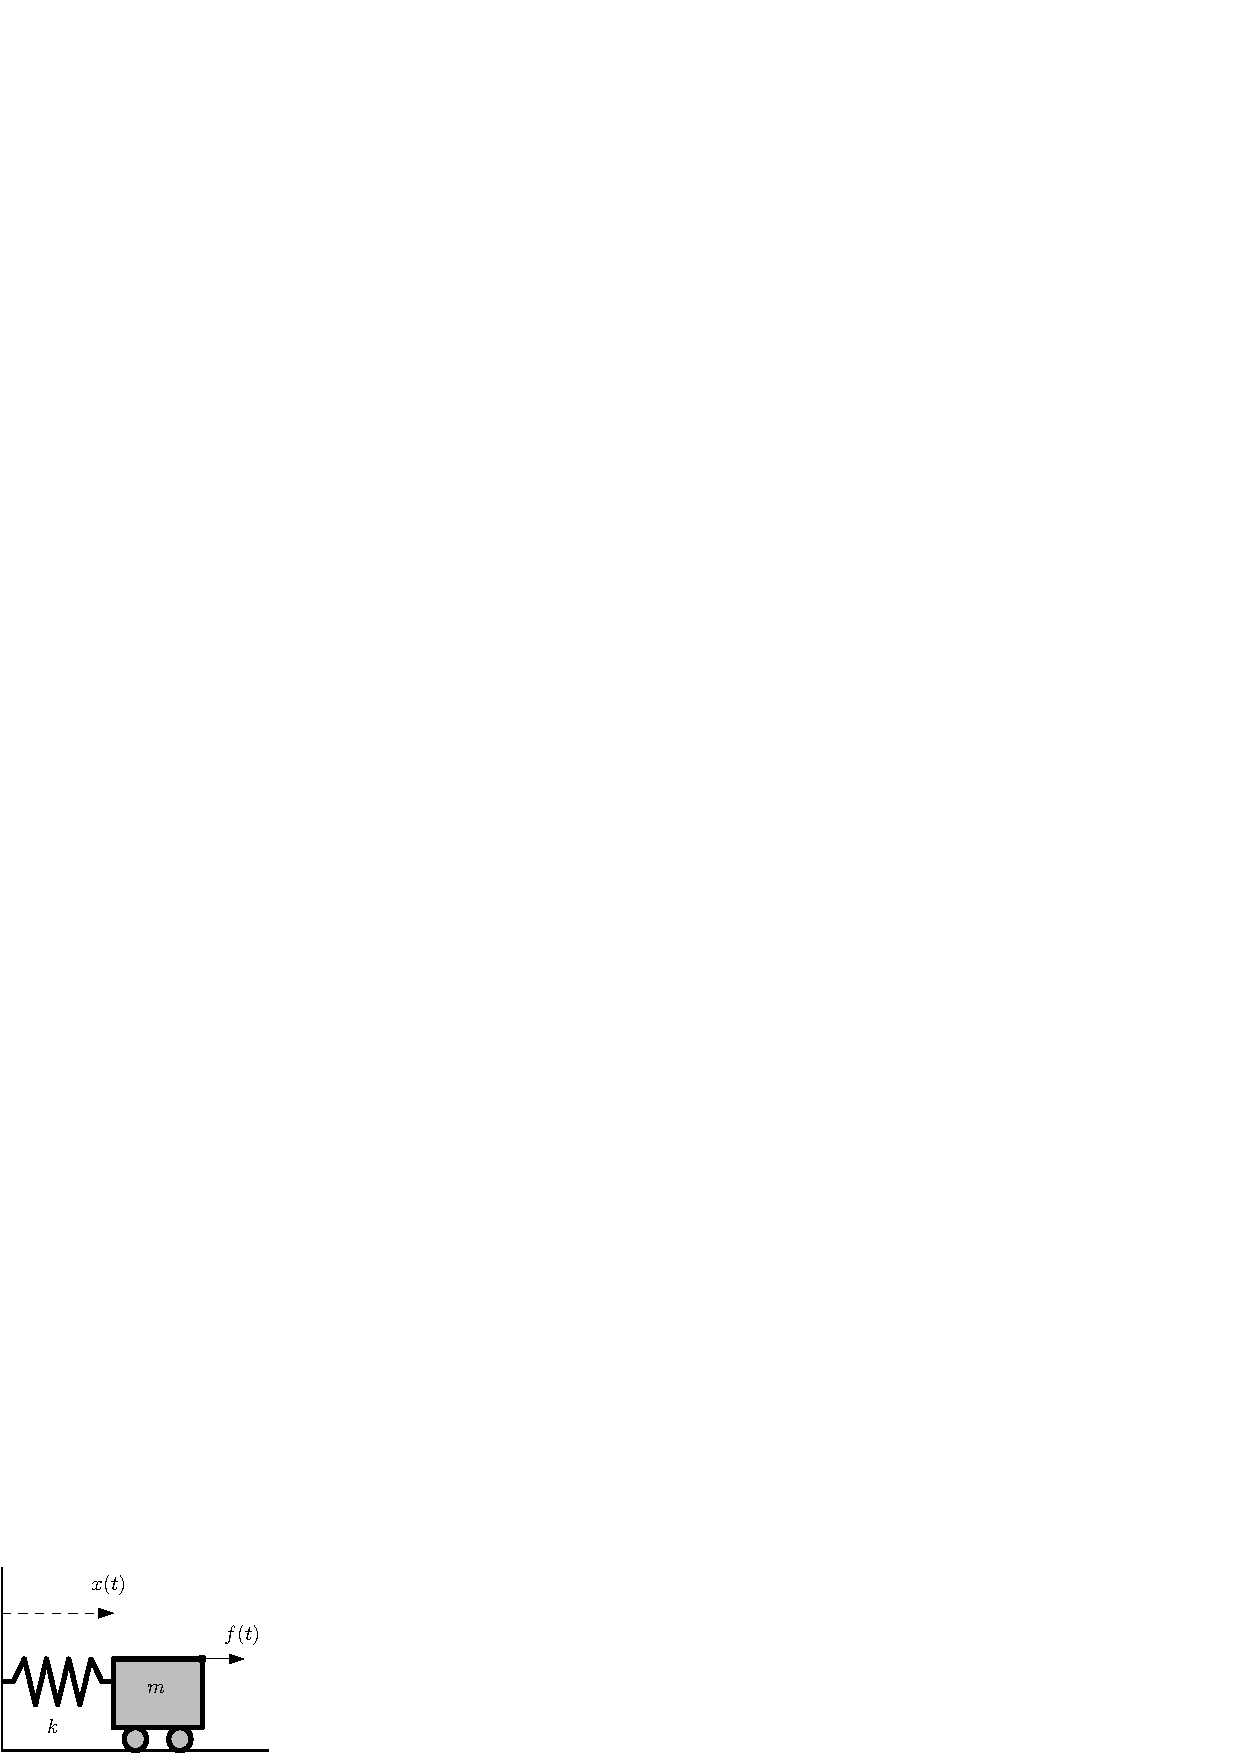
\includegraphics[width=0.75\linewidth]{figs/cart.png}
\end{marginfigure}
\begin{question}
  The figure in the margin shows a cart strapped by two elastic springs to walls. Sketch a free-body diagram for the cart and use it to write down the 2nd order \ode{} for position variable \(x\) using Newton's laws of motion. Leave \(f(t)\) as an unknown force function.
  \solspace{3in}
\end{question}

\newpage\begin{sagequestion}
  The \sage code in the link\footnote{Code for mass-damper-spring oscillator: \\ \url{https://goo.gl/p9EVdC}} computes solutions to the mass-damper-spring\index{mass-damper-spring} mechanical oscillator\index{oscillator} evolving from initial position \(p_{0}\) and initial velocity \(v_{0}\), given by equation:\index{damping}
  \begin{equation}
    \label{eq:w5-1}
    m \ddot x + c \dot x + k x = 0,\quad x(0)=p_{0}, \dot x(0) = v_{0}
  \end{equation}

  \begin{enumerate}[(a)]

  \item Copy the sketch into the graph below. Pay special attention to the
    points in which either of the functions intersects with the horizontal.

    \begin{minipage}{0.48\linewidth}
    \emptygrid{5}{4}
  \end{minipage}
    \begin{minipage}{0.48\linewidth}
  \item What is the position curve doing when the velocity curve intersects the horizontal?
  \solspace{0.25in}

\item Are these curves growing, decaying (transient), or neither? Are they oscillating or not?\index{transient}
  \solspace{0.25in}
\end{minipage}

\begin{minipage}{0.48\linewidth}
\item Slowly increase damping \(c\) by modifying the code until the curves stop oscillating. Try to find the smallest positive \(c\) that stops the oscillations. Then copy the graph into the space on the right and note the value of this \emph{critical damping}\index{damping!critical} \(c\).
\end{minipage} \begin{minipage}{0.48\linewidth}
\begin{center}
    \emptygrid{5}{4}

    \vspace{1em}
        Critical \(c = \)
    \end{center}
  \end{minipage}
\end{enumerate}

\end{sagequestion}

\begin{question}
  Verify that \(y(x) = e^{x}\sin(x)\) satisfies \(y''(x) - 2 y'(x) + 2 y(x) = 0\).
\end{question}
\solspace{3.5in}

\begin{question}
Given a linear \ode{} $y''= y' + 12y$. \index{characteristic equation!real roots}
\begin{enumerate}[(a)]
\item Is this equation homogeneous or not? How do you know? \index{homogeneous} \solspace{.25in}
\item Calculate the general solution of the \ode{}. \solspace{2in}
\item Calculate $c_1$ and $c_2$ so that $y(0) = 1$, and $y'(\pi) = 0$.\solspace{1.5in}
\end{enumerate}
\end{question}

\begin{question}
  Compute real and imaginary parts of each of the following expressions\footnote{
    Product of exponentials:
    \(e^{a\pm b} = e^{a} e^{\pm b}\)\\
    Euler's formula: \(e^{\pm i x} = \cos(x) \pm i \sin (x) \)
    }:
  \begin{enumerate}[(a)]
  \item \( \displaystyle (2+i)(3-i)\) \solspace{.5in}
    \item \( \displaystyle e^{3i}\) \solspace{.5in}
    \item \( \displaystyle e^{2-i\frac{\pi}{2}}\) \solspace{.5in} \marginnote{A consequence of Euler's formula\index{Euler's formula} is that the \(\cos\) and \(\sin\) functions can be defined using complex exponentials:
  \begin{align*}
    \cos(x) &= \frac{1}{2}e^{i x} + \frac{1}{2}e^{-i x} \\
    \sin(x) &= \frac{1}{2i}e^{i x} - \frac{1}{2i}e^{-i x}
  \end{align*}
Compare these formulas with those in the margin of the following page.}

    \item \( \displaystyle \frac{1}{i}\) \solspace{.5in}
    \item \( \displaystyle \frac{1}{1-i}\) \solspace{.5in}
  \end{enumerate}
\end{question}


\subsection*{Discussion Problems}

\begin{question}
  A particular solution to a second-order \ode{} is given by
  \[
    y(x) = 2e^{-3x} + 3 e^{x}
  \]

  \begin{enumerate}[(a)]
  \item Give the initial conditions \(y(0)\) and \(y'(0)\) of the function above.
  \item Give an example of a \ode{} whose solution is given by the function above.
\end{enumerate}
\end{question}

\begin{question}
  Calculate general solutions to the following linear \ode{}s, and particular solutions to IVPs where appropriate.
  \begin{enumerate}[(a)]
  \item \(\ddot{x} - 2\dot{x} - 3x = 0,\quad x(0) = 0, \dot x(0) = 1\)
  \item \(\ddot{y} - 5\dot{y} + 6y = 0,\quad y(0) = 1, \dot y(0) = -1\)
  \item \(y'''(x) - 3y''(x) + 2y'(x) = 0\)
  \end{enumerate}
\end{question}

\begin{question}
  Compute real and imaginary parts of each of the following numbers:
  \begin{colenumerate}[3]
    \item \(-2i(2+3i)\)
    \item \((1+i)(2+i)\)
    \item \((2-3i)(2+3i)\)
    \item \(e^{i \frac{\pi}{4}t}\)
    \item \(e^{2+i \frac{\pi}{4}}\)
    \item \(\frac{1}{2+i}  \)
  \end{colenumerate}
\end{question}

\subsection*{Additional practice problems}

\marginnote{Problems 4.3.38, 41 and 42 are significant. They discuss hyperbolic functions that have definitions similar to \(\cos\) and \(\sin\) in exponential form, except they do not use any complex numbers\index{hyperbolic functions}:
  \begin{align*}
    \cosh(x) &= \frac{1}{2}e^{x} + \frac{1}{2}e^{-x} \\
    \sinh(x) &= \frac{1}{2}e^{i x} - \frac{1}{2}e^{-x}
  \end{align*}
Compare these formulas with those in the margin of the previous page and notice that   \begin{align*}
    \cosh(ix) &= \cos(x) \\
    i \sinh(ix) &= \sin(x)
  \end{align*}}

\begin{colenumerate}
\item \smallcaps{Zill} \S 4.1.1--4, 29--34
\item \smallcaps{Zill} \S 4.1.38
\item \smallcaps{Zill} \S 4.3.1--14, 29--34
\item \smallcaps{Zill} \S 4.3.41--42
\end{colenumerate}
The problems where characteristic equation has complex or repeated roots will be covered on Wed and Fri. You can either wait until we cover these problems in lectures, or read ahead to see what happens in those cases.
%%% Local Variables:
%%% mode: latex
%%% TeX-master: "main"
%%% End:










\section{Complex and repeated roots,  Independence of solutions}

\begin{weekintro}
  Complex-valued functions\index{complex-valued functions} have real and imaginary parts, just like complex numbers. For functions, real and imaginary parts are functions themselves, that we can sketch. They often have related, but not identical, behaviors. \index{characteristic equation!complex roots}

  When roots of the characteristic polynomials repeat verbatim, such as in \(M^{2} + 2M + 1 = (M+1)^{2}\), we have to be careful in writing out the solution. These cases require a modification of the solution function in order to obtain the correct general solution.
  \index{characteristic equation!repeated roots}

\marginnote{\textbf{Definition} of a concept and \textbf{calculation} are not always equivalent in mathematics. Definition speaks of \emph{meaning}, while calculation tells us \emph{how to compute} something. For example, \emph{definition} of a solution of \(ax^{2} + bx + c = 0\) is ``any number that satisfies the equation'', and the calculation is given by the familiar quadratic formula. For quintic (5th order polynomial), there is no similar formula (calculation) of a solution, just a definition.}  Even though we infer very particular formulas for two functions that solve 2nd order linear \ode{}s, any two functions that are
  \begin{compactenum}[(i)]
    \item particular solutions (separately), and
    \item \textbf{linearly independent} \index{linear independence}
  \end{compactenum}
  can be used to form a general solution. What does it mean to be linearly independent? Informally, it means that behavior of one is fundamentally different from the other. A more in-depth definition is in the textbook. To \textbf{check} for linear independence, we use the Wronskian determinant.\index{Wronskian}
\end{weekintro}

\subsection*{Homework}


\begin{question}
  The complex-valued function\footnote{Notation \(e^{x} = \exp(x)\)}  \(f(t)\) depends on real variable \(t\):
  \[
f(t) =    \exp\left[(-1+i2\pi)t\right]
\]
\begin{enumerate}[(a)]
\item Compute the real part of the function \(\Re f(t)\) and the imaginary part \(\Im f(t)\). \solspace{1.5in}
  \item Sketch the real and imaginary parts for \(0 < t < 3\). Make sure to accurately represent growth/decay of each function, their value at \(t=0\), and points at which the functions intersect with the horizontal axis.

  \item For what values \(t\) is the function \(f(t)\) purely real (imaginary part is 0) and for what values is it purely imaginary (real part is \(0\))?

  \vspace{1em}

  \emptygrid{6}{2} \quad \emptygrid{6}{2}
\end{enumerate}
\end{question}

\begin{question}
  Compute solutions to the following linear homogeneous \ode{}s. In all cases, use real-valued formulas.
  \begin{enumerate}[(a)]
  \item \(y'' + 4y = 0\) \solspace{1in}
  \item \(y''+2y'+y = 0 \) \solspace{1in}
  \item \(y''+2y' + 5y = 0\) \solspace{1in}
  \end{enumerate}
\end{question}

\begin{question}
An unforced response of an oscillator can be modeled using the \ode{} \(m \ddot x(t) + c \dot x(t) + k x(t) = 0\), where \(m\) is the mass, \(c\) is the damping coefficient, and \(k\) the spring stiffness.\index{mass} \index{damping} \index{stiffness}
  \begin{enumerate}[(i)]
    \item  For \(m=4\) and \(k = 9\) and undetermined \(c \geq 0\), find the roots of the characteristic equation. \solspace{1in}
    \item Find the ranges of values of \(c\) such that the general solution is:
      \begin{inparaenum}[(i)]
      \item decaying and shows no oscillation,
      \item decaying and has oscillations.
      \end{inparaenum} Compare your answer here to the \sage problem in previous week's homework.

      \solspace{1in}
    \item Choose one value for each range you determined and write out the formula for the general solution. \solspace{2in}
    \end{enumerate}
    \solspace{4in}
\end{question}

\subsection*{Discussion Problems}

\begin{question}
  Calculate real and imaginary parts of the following functions (\(t\) is always a real number):
  \begin{colenumerate}[3]
  \item \((2+i)\cos(t)\)
  \item \(3i[ \cos(t) - i\sin (t) ]\)
  \item \(\exp( i2t )\)
  \item \((2+i)\exp( i2t )\)
  \item \(\exp(3t-i2t )\)
  \item \(5e^{(2+i \frac{\pi}{4})t}\)
  \end{colenumerate}
\end{question}

\begin{question}
Given $y''-2y'+2y = 0$.
\begin{enumerate}[(a)]
\item Verify that $y=c_1e^x\cos(x) + c_2 e^x\sin(x)$ is a general solution to the given \ode{}.
\item Find $c_1$ and $c_2$ so that $y(0) = 1$, and $y'(\pi) = 0$.
\item Use Wronskian to verify that $e^{x}\cos(x)$ and $e^{x}\sin(x) $ are linearly independent.
\end{enumerate}
\end{question}

\begin{question}
Find the general (or particular) solution and determine if the solution will exhibit growth or decay.\index{growth} \index{decay}
\begin{colenumerate}
\item $y''+8y'+16y = 0$
\item $y''+2y'+2y = 0$
\item $y''+2y'-8y = 0$, $y(0) = 7$, $y'(0) = 2$
\end{colenumerate}
\end{question}

\begin{question}
  For each of the following pairs of numbers:
  \begin{itemize}
  \item find quadratic equations with real coefficients that have the following roots,
  \item describe (oscillating or not, growing/decaying/neither) the shape of solutions of a 2nd order linear \ode{} whose characteristic equation would be given by the quadratic you just found.
  \end{itemize}
    \begin{colenumerate}[4]
    \item \(-2\), \(3\)
    \item \(0\), \(2\)
    \item \(2\), \(2\)
    \item \(\pm i\)
    \item \(2 \pm i\)
    \item \(A, B\)
    \item \(A \pm i B\)
    \end{colenumerate}
where \(A, B\) are both real constants.
\end{question}

\begin{question}
  For each of the functions below
  \begin{compactitem}
  \item Give the initial conditions \(y(0)\) and \(y'(0)\) of the function above.
  \item Give an example of a \ode{} whose solution is given by the function above.
  \end{compactitem}

  \begin{colenumerate}[2]
  \item \(y(x) = 2e^{-3x} + 3 e^{x}\)
  \item \(y(x) = \sin(x) + \cos(x)\)
  \item \(y(x) = xe^{-2x} -3 e^{-2x}\)
  \item \(y(x) = e^{-x}\cos(2x)\)
  \end{colenumerate}
\end{question}


\begin{question}
A mass of  \(4 \si{kg}\) is attached to a spring whose spring constant is 16 \si{kg/s^2}. What is the period of the motion of the mass when it is allowed to bounce freely?
\end{question}

\begin{question}
A mass of \(20 \si{kg}\) is attached to a spring. If the frequency of its free motion is $2/\pi$ cycles/s,
what is the spring constant $k$? What is the frequency of free motion if the original mass is replaced with an \(80 \si{kg}\) mass?
\end{question}

\subsection*{Additional practice problems}

\begin{compactenum}[(a)]
\item \smallcaps{Zill} \S 4.1.15--19 (Wronskian, independence of solutions)
\item \smallcaps{Zill} \S 4.3.1--14, 29--34, 41--42 (homogeneous \ode{}s)
\item \smallcaps{Zill} \S 5.1.1--12, 17--23 (mass-spring-damper models)
\end{compactenum}

%%% Local Variables:
%%% mode: latex
%%% TeX-master: "main"
%%% End:



\section{Undetermined coefficients}

\begin{weekintro}
  While characteristic equations are extremely useful for solving homogeneous \ode{}s, they do not help much when solving the inhomogeneous subproblem.\index{inhomogeneous}

  \emph{Undetermined coefficients}\index{undetermined coefficients} is a technique for making \textbf{educated guesses} about \textbf{candidates} for the inhomogeneous solutions. These candidates have undetermined parameters in them that are computed by plugging the candidate into the DiffEq.

  \textbf{Rely as little as possible on tables of undetermined coefficients.} Instead focus on three principles:
  \begin{itemize}
  \item If the input function is a sum of terms, then we can solve inhomogeneous equations with each of the terms in the sum in isolation, and add their solutions together.
  \item A good candidate for an inhomogeneous solution is formed by a linear combination of derivatives of the input function.
  \item If the candidate for inhomogeneous solution matches a component in the \emph{homogeneous} solution, multiply the candidate by the independent variable (repeat if necessary).
  \end{itemize}

In a particular case of undamped oscillators, the third principle above corresponds to the \textbf{resonance}: growth of the output despite bounded input.
\end{weekintro}

\subsection*{Homework}

\begin{question}
  For each of the following, determine the homogeneous solution and the \textbf{form} of a particular non-homogeneous solution:
  \begin{fullwidth}
  \begin{colenumerate}[4]
  \item \(y'' + 4y = x^{2}\)
  \item \(y'' + 4y = 10 + \sin(x)\)
  \item \(y'' + 4y = \sin(2 x)\)
  \item \(y'' + 4y = e^{x}\sin(2 x)\)
\end{colenumerate}
  \solspace{1in}
\end{fullwidth}
\end{question}

\begin{question}
For the differential equation
  \[
    y'' + 9y = x + \sin(x)
  \]
  \begin{enumerate}[(i)]
  \item Solve
    \begin{fullwidth}
    \begin{colenumerate}[3]
    \item Homog. Subproblem
    \item Inhomog. Subproblem 1
    \item Inhomog. Subproblem 2
    \end{colenumerate}

    \solspace{3in}

    \end{fullwidth}
    \item General solution using part (i). \solspace{0.5in}
  \item Particular solution that satisfies \(y(0)=1\), \(y'(0) = 0\). \solspace{2in}
  \end{enumerate}
\end{question}

\begin{question}
A mass of \(24 \si{kg}\), attached to the end of a spring of unknown coefficient \(k\), stretches it \(4\si{cm}\) under influence of gravity (\(g \approx 10 \si{ms^{-2}}\)) when the mass is not moving.
\begin{enumerate}[(i)]
  \item Write the differential equation for the system.
  \item Compute the equilibrium solution for the equation and determine spring coefficient from it.
  \item Initially, the mass is released from rest from a point \(3 \si{cm}\) above the equilibrium position. Find the particular solution of the differential equation.
\item In a second scenario, a periodic force \(\cos(\Omega t)\) is applied to the mass in addition to gravity. What is the value of frequency \(\Omega\) which excites resonance\index{resonance} in the motion of the weight?
\end{enumerate}
\end{question}

\begin{sagequestion}
  The \sage code in the link is the same as used a couple of weeks ago.\footnote{Code for mass-damper-spring oscillator: \\ \url{https://goo.gl/p9EVdC}} Modify the code so that it corresponds to the differential equation
  \begin{equation}
    \label{eq:w7-1}
    \ddot x + 4 x = \sin( \Omega t ),\quad x(0)=p_{0}, \dot x(0) = v_{0}
  \end{equation}
  by changing the line 10 appropriately. \footnote{To represent symbol \(\Omega\) you can add a variable \texttt{Omega} in the same fashion as \texttt{mass}, \texttt{damping}, etc. are defined. Set \(\Omega=1\) initially.}
  \begin{enumerate}[(a)]

  \item Copy the sketch for \(\Omega=1\) into the graph below. \footnote{Set \texttt{xmax=20} in lines 22 and 28 and \texttt{ymin=-10} and \texttt{ymax=20} at the end of the code to show you the full extent of solution curves.}

    \begin{minipage}{0.48\linewidth}
    \emptygrid{5}{4}
  \end{minipage}
    \begin{minipage}{0.48\linewidth}
  \item Describe how the graphs are different compared to the graphs without \(\sin(\Omega t)\) added (you can look back to Week 5).
  \solspace{0.25in}

\item Are these new curves growing, decaying, or neither? Are they oscillating or not?
  \solspace{0.25in}
\end{minipage}
\item Write down the characteristic equation and find its roots. What is the value of the \emph{resonant frequency} of this oscillator?
  \solspace{.5in}

\begin{minipage}{0.48\linewidth}
\item Set \(\Omega\) equal to the \emph{resonant frequency}\index{resonant frequency} of the differential equation. Then copy the graph into the space on the right.

  Resonant \(\Omega = \)
\end{minipage} \begin{minipage}{0.48\linewidth}
  \begin{center}
    Resonant \(\Omega = \)

    \emptygrid{5}{4}

    \vspace{1em}
        Are the curves growing, decaying, or neither? \index{resonance}
    \end{center}
  \end{minipage}
\end{enumerate}

\end{sagequestion}


\subsection*{Discussion and Practice Problems}

\begin{question}
  In each of the following equations, undetermined coefficient candidate for the inhomogeneous solution is incorrectly proposed.
  \begin{compactitem}
  \item Proceed with the incorrect candidate and \textbf{show how the solution process fails}.
  \item \textbf{Propose the correct undetermined coefficients candidate}.
  \item \textbf{Find the coefficients} of the inhomogeneous solution.
  \end{compactitem}
 \begin{enumerate}[(a)]
  \item \(y'' + 2y' + 5y = x^{2}\), incorrect candidate: \(y_{p}(x) = A x^{2} + B\)
  \item \(y'' + 9 y = \sin(x)\), incorrect candidate: \(y_{p}(x) = A \sin(x)\)
  \item \(y'' + 9 y = \sin(3x)\), incorrect candidate: \(y_{p}(x) = A \cos(3x) + B\sin(3x)\)
\end{enumerate}
\end{question}

\begin{question}
For each of the following, determine the homogeneous solution and the \textbf{form} of a particular non-homogeneous solution:
  \begin{colenumerate}
  \item $y''+3y'+2y = -10x^2$
  \item $y''+3y'+2y =e^{4x}$
  \item $y''+2y'=x^2+5x$
  \item $y''+4y'+13y = 2xe^{-2x}\sin(3x)$
  \item $y''+2y'+2y=5e^{-x}\cos(x)$
  \item $y''+6y'+9y = x^3e^{-3x}$
  \end{colenumerate}
\end{question}

\begin{question}
Using the method of undetermined coefficients to find the general solution:
  \begin{enumerate}[(i)]
  \item $y''+3y'+2y=-10x^2$
  \item $y''+3y'+2y =e^{4x}$
  \item $y''+y'-2y = 20\sin(2x)$
  \item $y'''-2y''+y' = 2-24 e^x +40 e^{5x}$, $y(0) = 1/2, y'(0)=5/2, y''(0) = -9/2$.
  \end{enumerate}
\end{question}

\begin{question}
A weight of \(8 \si{kg}\) hung from a spring stretches the spring \(3\si{cm}\). The mass-spring system is additionally encumbered by air resistance, which is proportional to velocity with coefficient \(1 \si{kg/s}\). The mass moves under the influence of gravity (\(g \approx 10 ms^{-2}\)) and an external force of $10\cos(4t) \si{kgms^{-2}}$ (t is seconds
after the release). If the weight is pulled down \(1 \si{m}\) from its equilibrium position
and given an initial upward velocity of \(2 \si{m/s}\), write an initial value problem for the position of
the object at time t seconds and solve.
\end{question}

\subsection*{Additional practice problems}


\begin{colenumerate}
  \item \smallcaps{Zill} \S 4.4.1--15, 27--32 (undet. coeff)
  \item \smallcaps{Zill} \S 5.1.29--34 (forced oscillator)
  \item \smallcaps{Zill} \S 5.1.37--38 (resonance)
\end{colenumerate}
%%% Local Variables:
%%% mode: latex
%%% TeX-master: "main"
%%% End:
